
\section{Training Curves}\label{sec:graphs:training_curves}

Both \textit{katz-eig} and \textit{link-analysis} are iterative algorithms. Their descriptions use the phrase "repeat until convergence".  With training curves, which plots the evaluation metric with the respect to epochs, the number of iterations, the effect of running more iterations can be seen.

The plots have recommendations calculated using the training set and evaluated against the training set for \textit{Precision}, \textit{Recall} and \textit{F-measure} using the top-10 recommendations. Each $K$ are different for each dataset, using a learned optimal value, and $beta = \frac{1}{\|A_{train}\|_2}$.

\subsection{katz-eig}

\FloatBarrier

\begin{figure}[h!]
\centering
\begin{minipage}{.5\textwidth}
    \centering
    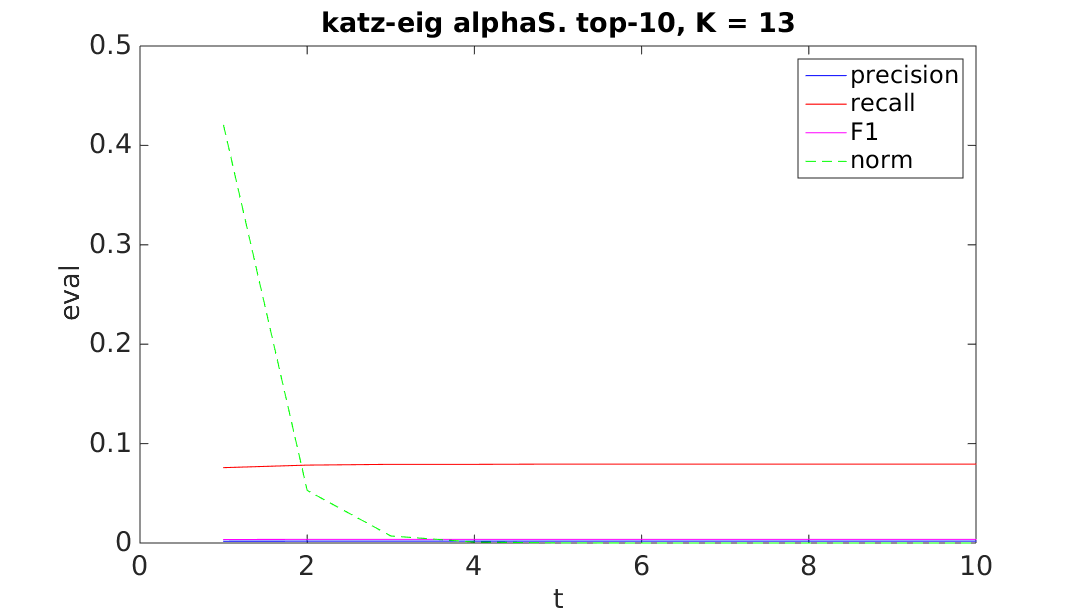
\includegraphics[width=\linewidth]{fig/katzeig_t/alphaS_katzeig_t.png}
    \captionof{figure}{\textit{alphaS}}
\end{minipage}%
\begin{minipage}{.5\textwidth}
    \centering
    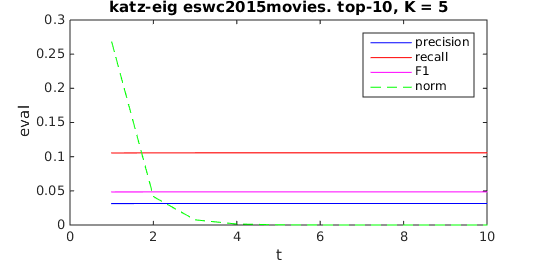
\includegraphics[width=\linewidth]{fig/katzeig_t/eswc2015movies_katzeig_t.png}
    \captionof{figure}{\textit{eswc2015movies}}
\end{minipage}
\end{figure}

\begin{figure}[h!]
\centering
\begin{minipage}{.5\textwidth}
    \centering
    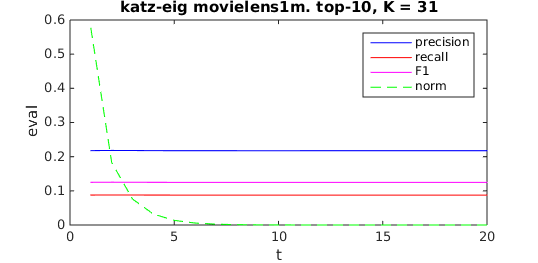
\includegraphics[width=\linewidth]{fig/katzeig_t/movielens_katzeig_t.png}
    \captionof{figure}{\textit{movielens1m}}
\end{minipage}%
\begin{minipage}{.5\textwidth}
    \centering
    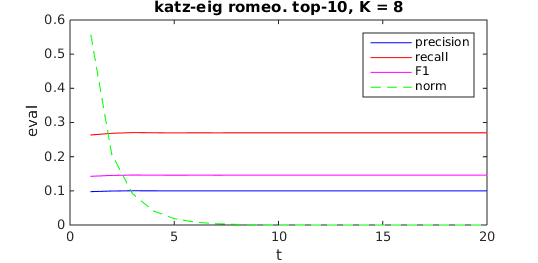
\includegraphics[width=\linewidth]{fig/katzeig_t/romeo_katzeig_t.png}
    \captionof{figure}{\textit{romeo}}
\end{minipage}
\end{figure}

\FloatBarrier

The jagged line represents $\|S_t - S_{t - 1}\|_2$, which is a measure of the difference between the current iteration $t$ and the previous iteration. This was made as a measure of the convergence criteria. Convergence was reached with relatively few iterations, but the matrix $S$ is small and the calculation has low complexity.

In all following usages of \textit{katz-eig}, a value of $\epsilon = 0.01$ was used to break iterations if $\|S_t - S_{t - 1}\|_2 < \epsilon$.

\newpage


\subsection{link-analysis}

\begin{figure}[h!]
\centering
\begin{minipage}{.5\textwidth}
    \centering
    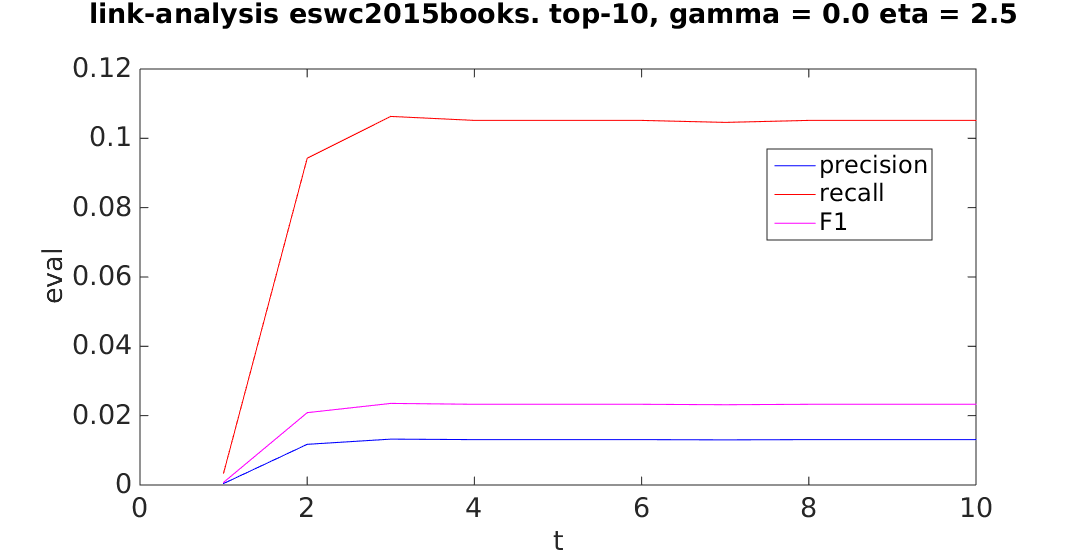
\includegraphics[width=\linewidth]{fig/link_t/eswc2015books_link_t.png}
    \captionof{figure}{\textit{eswc2015books}}
\end{minipage}%
%\begin{minipage}{.5\textwidth}
    %\centering
    %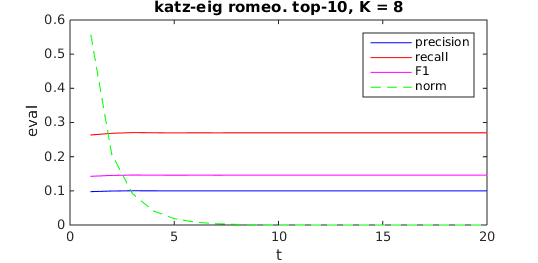
\includegraphics[width=\linewidth]{fig/katzeig_t/romeo_katzeig_t.png}
    %\captionof{figure}{\textit{romeo}}
%\end{minipage}
\end{figure}

\Warning[TODO]{ More plots }

For \textit{link-analysis} convergence is also fast. The choice here was to fix $t_{max}$ to a fixed value instead of measuring convergence either by calculating $\| \PR_t - \PR_{t - 1} \|_2$
or by explicitly calculating \textit{F-measure} and measuring the change. This was done because the iteration step in \textit{link-analysis}, in contrast to \textit{katz-eig}, handles large matrices and calculations such as these would be time consuming.

In all following usages of \textit{link-analysis}, the iteration count was fixed to $t_{max} = 3$.

